\chapter{Spanning Trees}
Rishnak found Ajur and Jura walking along a stretch of road with trees on either side. Recalling his previous talks with Ajur about trees, Rishnak chose a specific kind of tree that is found within a graph for his next session with Ajur.

Rishnak said, ``A graph~$G$ is connected if there is a path between every pair of vertices in~$G$. So, in connected graph~$G=(V,E)$, a \textit{spanning tree} is tree~$T(V,E_1)$ that covers all vertices in~$V$ and is a subgraph of~$G$ that satisfies two conditions:
\begin{enumerate}
    \item Subgraph~$T$ is a tree, meaning it contains no cycles and is connected.
    \item Vertex set~$V$ of~$T$ is the same as that of~$G$.''
\end{enumerate}

Rishnak flashed his hands and formed two graphs in the air in front of Ajur [Figure~\ref{11g1}] [Figure~\ref{11g2}]. He said, ``Here is an example of a graph with a corresponding spanning tree.''

\begin{figure}
\begin{center}
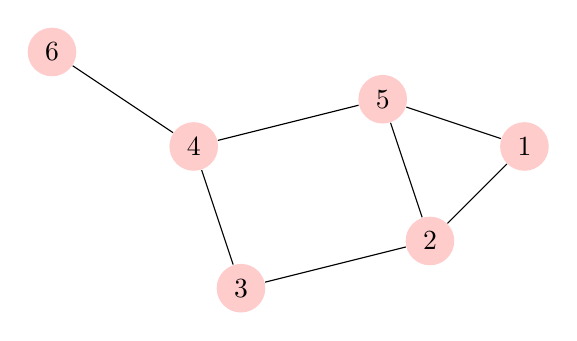
\begin{tikzpicture}
  [scale=.6,auto=left,every node/.style={circle,fill=red!20}]
  \node (n6) at (1,10) {6};
  \node (n4) at (4,8)  {4};
  \node (n5) at (8,9)  {5};
  \node (n1) at (11,8) {1};
  \node (n2) at (9,6)  {2};
  \node (n3) at (5,5)  {3};

  \foreach \from/\to in {n6/n4,n4/n5,n5/n1,n1/n2,n2/n5,n2/n3,n3/n4}
    \draw (\from) -- (\to);

\end{tikzpicture}
\caption{Example graph with six vertices and seven edges}\label{11g1}
\end{center}
\end{figure}

\begin{figure}
\begin{center}
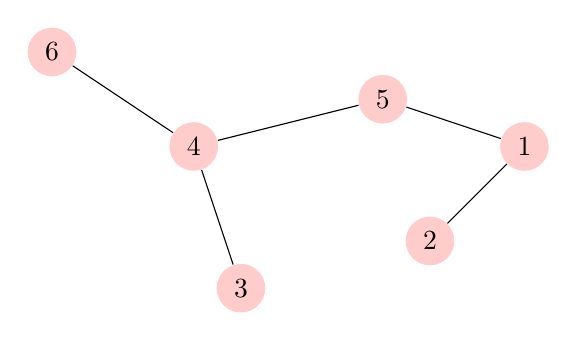
\begin{tikzpicture}
  [scale=.6,auto=left,every node/.style={circle,fill=red!20}]
  \node (n6) at (1,10) {6};
  \node (n4) at (4,8)  {4};
  \node (n5) at (8,9)  {5};
  \node (n1) at (11,8) {1};
  \node (n2) at (9,6)  {2};
  \node (n3) at (5,5)  {3};

  \foreach \from/\to in {n6/n4,n4/n5,n5/n1,n1/n2,n3/n4}
    \draw (\from) -- (\to);

\end{tikzpicture}
\caption{A subgraph of the graph shown in Figure~\ref{11g1} that forms a spanning tree of the original graph}\label{11g2}
\end{center}
\end{figure}

Ajur studied both graphs, recognizing that the second graph was a subgraph of the first.

Rishnak asked Ajur if he could construct another spanning tree for the original graph [Figure~\ref{11g1}].

Ajur was eager to show off and drew a subgraph in the dirt with a stick [Figure~\ref{11g3}].

\begin{figure}
\begin{center}
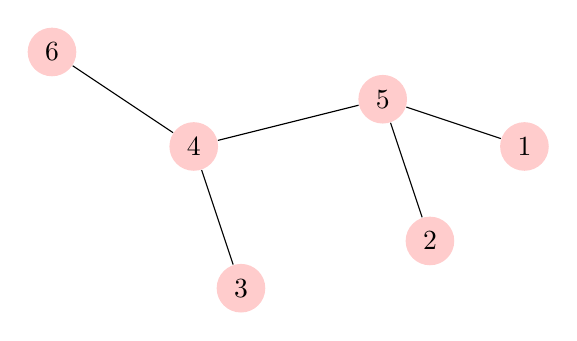
\begin{tikzpicture}
  [scale=.6,auto=left,every node/.style={circle,fill=red!20}]
  \node (n6) at (1,10) {6};
  \node (n4) at (4,8)  {4};
  \node (n5) at (8,9)  {5};
  \node (n1) at (11,8) {1};
  \node (n2) at (9,6)  {2};
  \node (n3) at (5,5)  {3};

  \foreach \from/\to in {n6/n4,n4/n5,n5/n1,n2/n5,n3/n4}
    \draw (\from) -- (\to);

\end{tikzpicture}
\caption{Another spanning tree of the graph shown in Figure~\ref{11g1}}\label{11g3}
\end{center}
\end{figure}

Rishnak asked, ``How many distinct spanning trees are there?''

Ajur thought about this for a moment. He said, ``Do you mean how many labeled non-isomorphic trees there are?''

Rishnak said, ``Yes, exactly the question?''

Ajur said, ``There are two cycles in this graph, namely~$(2,3,4,5)$ and~$(1,2,5)$, and they share common edge~$(2,5)$. The cycles are of length~4 and length~3, so there are four possible spanning trees to choose from out of the first cycle and three possible spanning trees to choose from out of the other cycle. Multiply these together and we have~12 possibilities, but one of them ends up being cycle~$(1,2,3,4,5)$ if edge~$(2,5)$ is omitted. Therefore, we have~11 spanning trees, each of which must also contain edge~$(4,6)$. Here they are.''

Ajur painstakingly wrote out all~11 spanning trees in the dirt as follows:
\begin{enumerate}
    \item \{(4,6),(4,5),(5,2),(2,3),(5,1)\}
    \item \{(4,6),(4,5),(5,2),(2,3),(2,1)\}
    \item \{(4,6),(4,5),(4,3),(5,2),(5,1)\}
    \item \{(4,6),(4,5),(4,3),(5,2),(2,1)\}
    \item \{(4,6),(4,3),(2,3),(5,2),(5,1)\}
    \item \{(4,6),(4,3),(2,3),(5,2),(2,1)\}
    \item \{(4,6),(4,5),(4,3),(2,3),(5,1)\}
    \item \{(4,6),(4,5),(4,3),(2,3),(2,1)\}
    \item \{(4,6),(4,5),(2,3),(5,1),(1,2)\}
    \item \{(4,6),(4,5),(4,3),(5,1),(1,2)\}
    \item \{(4,6),(4,3),(3,2),(2,1),(1,5)\}
\end{enumerate}

Rishnak nodded and started to speak, but Ajur asked, ``What about the maximum number of labeled spanning trees in a graph with~$n$ vertices? For a complete graph, it must be the maximum number of edges in a graph with~$n$ vertices.''

Rishnak said, ``Correct. Complete graphs have the largest possible number of spanning trees. We can find the number of spanning trees in a complete graph using Pr{\"u}fer codes, which we talked about a few days ago.\footnote{See their discussion in Chapter~8}

Ajur remembered Pr\"ufer codes and said, ``For a tree with~$n$ vertices, we need a Pr{\"u}fer code of length~$n-2$. Each of the~$n-2$ characters in the code could be any of the~$n$ vertices. Therefore, the number of labeled spanning trees in a complete graph with~$n$ vertices has to be~$n^{(n-2)}$.''

Rishnak smiled, then said, ``In general, since there are~$n-1$ edges in a spanning tree, each of the remaining~$e-n+1$ edges, when added to the spanning tree will necessarily create a cycle. Therefore, we will have~$e-n+1$ cycles in the given graph. These cycles are called \textit{fundamental cycles} and, as I have just described, each fundamental cycle has exactly one non-spanning tree edge.\footnote{Euler's equation~(\ref{eqn:euler}) back in Chapter~9 uses this fact.} Let me show you.''

Rishnak waved his hands and the original graph appeared with its edges glimmering in red and blue [Figure~\ref{11g4}]. Rishnak said, ``The blue edges are spanning tree edges, whereas the red edges are non-spanning tree edges that each form a fundamental cycle.''

\begin{figure}
\begin{center}
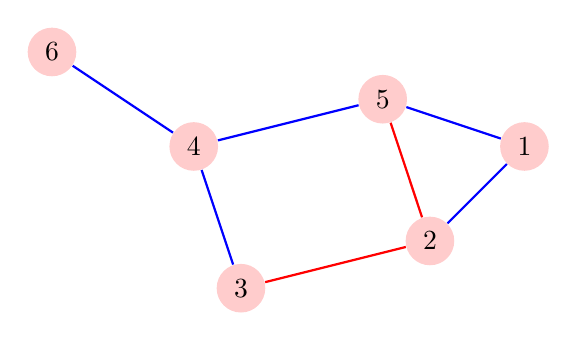
\begin{tikzpicture}
  [scale=.6,auto=left,every node/.style={circle,fill=red!20}]
  \node (n6) at (1,10) {6};
  \node (n4) at (4,8)  {4};
  \node (n5) at (8,9)  {5};
  \node (n1) at (11,8) {1};
  \node (n2) at (9,6)  {2};
  \node (n3) at (5,5)  {3};

  \foreach \from/\to in {n6/n4,n4/n5,n5/n1,n1/n2,n3/n4}
    \draw [thick,color=blue] (\from) -- (\to);
  \foreach \from/\to in {n5/n2,n2/n3}
   \draw [thick,color=red] (\from) -- (\to);
\end{tikzpicture}
\caption{Original graph from Figure~\ref{11g1} with respect to the spanning tree shown in Figure~\ref{11g2}; here, spanning tree edges are shown as thick blue lines while non-spanning tree edges are shown in red, the latter forming fundamental cycles~$(1,2,5)$ and~$(3,4,5,1,2)$}\label{11g4}
\end{center}
\end{figure}

Ajur wanted to better understand how to find a spanning tree for a given graph, so he asked Rishnak about this.

Rishnak smiled and said, ``First, the graph has to be connected. If that's the case, then it can be done using the following steps:
\begin{enumerate}
\item Start from any vertex. Add that vertex to empty set~$S$.
\item From the vertices in~$S$, find a vertex~$v$ that is not in~$S$ that is adjacent to one of the vertices~$w$ in~$S$. Add that edge~$(v,w)$ to spanning tree~$T$.
\item Repeat Step~2 until all vertices are in~$S$.''
\end{enumerate}

Rishnak formed the original graph again in the air in front of Ajur [Figure~\ref{11g1}]. He said, ``Let me illustrate this. First, add vertex~1 to the set. It has adjacent vertices~2 and~5. Let's say we choose vertex~5 and add it to~$S$. Edge~$(1,5)$ is then the first edge of our spanning tree. From vertices in~$S$, we pick a vertex that is adjacent but not already in~$S$. Choices here are vertices~2 or~4. Let's say we choose vertex~2 and therefore include edge~$(1,2)$ in the spanning tree.''

Ajur said, ``We could have also included edge~$(5,2)$ instead of~$(1,2)$ in the spanning tree, right?''

Rishnak said, ``Yes, the choice is arbitrary. Now, at this point, we have~$S=(1,2,5)$. So we find a vertex not in~$S$ that is adjacent to any of these three vertices. There are two vertices to choose from, namely vertices~3 and~4. Let's say we choose vertex~4 and therefore include edge~$(4,5)$ in the spanning tree.''

Ajur chimed in, ``Now vertices~$(1,2,4,5)$ are in set~$S$. From these vertices, we find a vertex that is adjacent but not in~$S$, so we're looking at vertices~3 and~6. If we choose vertex~3, then we include edge~$(4,3)$ in the spanning tree. Repeating this one more time, we choose vertex~6 and include edge~$(4,6)$ in the spanning tree. And now we're done!''

Rishnak nodded and said, ``Right, now set~$S$ contains all of the vertices, and we have spanning tree~$T$ with edges~$(1,5)$, $(1,2)$, $(5,4)$, $(4,3)$, and $(4,6)$.''---Rishnak waved his hands and the spanning tree from earlier appeared [Figure~\ref{11g2}]---``This is the same spanning tree we came up with earlier.''

Ajur nodded eagerly. He said, ``Aha, and if we had made different choices along the way, we would have ended up with a different spanning tree, like this one.''---Ajur quickly drew another spanning tree in the dirt [Figure~\ref{11g3}].

Rishnak smiled, happy to see that Ajur understood. He said, ``Here is another interesting problem related to spanning trees. As background, a graph is called a \textit{weighted graph} if there are numeric weights or costs associated with each edge. The weight could represent the distance in miles or the cost of travel, and so on.''

Rishnak flashed his hands and the original graph [Figure~\ref{11g1}] appeared, this time with numeric values next to each edge [Figure~\ref{11g7}]. He said, ``Here is an example weighted graph. See each weighted edge?''

\begin{figure}
\begin{center}
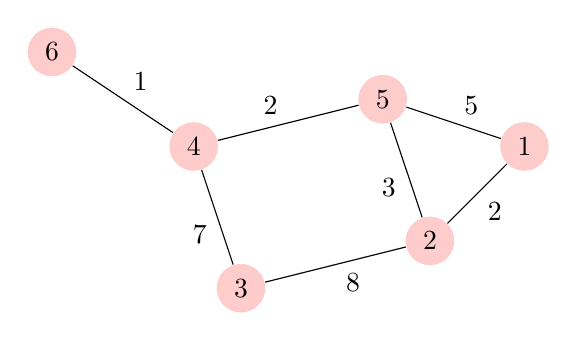
\begin{tikzpicture}
  [scale=.6,auto=left,every node/.style={circle,fill=red!20}]
  \tikzstyle{weight} = [fill=none]
  \node (n6) at (1,10) {6};
  \node (n4) at (4,8)  {4};
  \node (n5) at (8,9)  {5};
  \node (n1) at (11,8) {1};
  \node (n2) at (9,6)  {2};
  \node (n3) at (5,5)  {3};
  \foreach \source /\dest /\weight in {n6/n4/1,n4/n5/2,n5/n1/5,n1/n2/2,n2/n5/3,n2/n3/8,n3/n4/7} 
   \draw (\source) --node[weight] {$\weight$}  (\dest);
\foreach \source /\dest /\weight in {1/3/1} place \weight above of=\path;
  
  \end{tikzpicture}
\caption{The graph shown in Figure~\ref{11g1} with edge weights associated with each edge}\label{11g7}
\end{center}
\end{figure}

Ajur said, ``Yes, but how does this change our spanning tree problem?''

Rishnak saw Ajur's impatience. He said, ``We want to find a \textit{minimum spanning tree} in which the sum of all edge weights in the spanning tree is the smallest possible.''

Ajur said, ``Aha, we can enumerate all spanning trees and for each such spanning tree, compute the sum of the edge weights, then choose the spanning tree with the smallest sum.''

Rishnak smiled and said, ``That will work, though that is what we call a \textit{brute force} method. It can be a good strategy for many problems, but we can often find more efficient methods. In this case, we would like to find a faster method that makes certain choices such that we do not have to consider all possible spanning trees.''

Ajur frowned and said, ``I see. If the graph was much larger, we'd have a lot of work to do if we used a brute force approach.''

Rishnak said, ``Exactly. Do not despair, though. We can modify Step~2 of the procedure that I already described to better select each edge. Here is the modified approach:
\begin{enumerate}
\item Start from any vertex. Add that vertex to empty set~$S$.
\item From the vertices in~$S$, find a vertex~$v$ that is not in~$S$ that is adjacent to one of the vertices~$w$ in~$S$---but make sure that edge~$(v,w)$ has the smallest possible edge weight at that decision point. Add that edge~$(v,w)$ to minimum spanning tree~$T$.
\item Repeat Step~2 until all vertices are in~$S$.''
\end{enumerate}

Ajur decided to work through an example by using the graph that Rishnak had formed in front of him [Figure~\ref{11g7}]. He first drew the vertices of the graph in the dirt. Next, he chose vertex~1 and added it to set~$S$. From the two possible edges incident at vertex~1, he chose vertex~2 and added it to~$S$ since the edge weight for edge~$(1,2)$ was smaller than that of edge~$(1,5)$.

Ajur said, ``Aha, I see! Now that vertices~1 and~2 are in~$S$, of the edges leaving~$S$, edge~$(2,5)$ has the smallest edge weight. Therefore, edge~$(2,5)$ is added to the minimum spanning tree and vertex~5 is added to~$S$. Then, from vertices in~$S$, namely~1, 2 and~5, edge~$(5,4)$ has the smallest edge weight. And this continues until we visit each vertex, which we know by adding each vertex in turn to set~$S$.''---Ajur drew each edge in the dirt as he followed the algorithm through to its end [Figure~\ref{11g8}]---``Set~$S$ contains all of the vertices, so here's the minimum spanning tree!''

\begin{figure}
\begin{center}
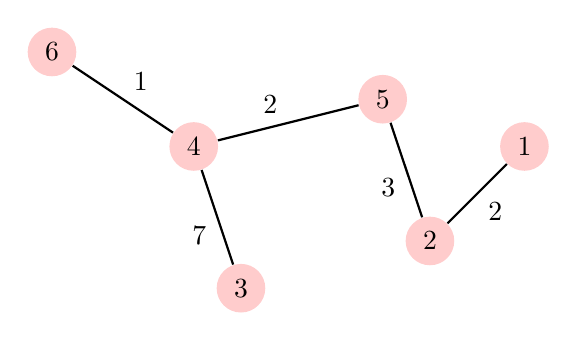
\begin{tikzpicture}
  [scale=.6,auto=left,every node/.style={circle,fill=red!20}]
  \tikzstyle{weight} = [fill=none]
  \node (n6) at (1,10) {6};
  \node (n4) at (4,8)  {4};
  \node (n5) at (8,9)  {5};
  \node (n1) at (11,8) {1};
  \node (n2) at (9,6)  {2};
  \node (n3) at (5,5)  {3};
  \foreach \source /\dest /\weight in {n6/n4/1,n4/n5/2,n1/n2/2,n2/n5/3,n3/n4/7} 
   \draw[thick] (\source) --node[weight] {$\weight$}  (\dest);
\foreach \source /\dest /\weight in {1/3/1} place \weight above of=\path;
  
  \end{tikzpicture}
\caption{A minimum spanning tree with a total weight of~15 for the weighted graph given in Figure~\ref{11g7}}\label{11g8}
\end{center}
\end{figure}

Rishnak laughed as Ajur could barely control his enthusiasm. Ajur exclaimed, ``We could also use this algorithm to minimally connect a given set of points in a plane. Vertices would correspond to the points. And the distances between each of these points could simply be the length of the straight lines joining them.''

Ajur showed his work in Figure~\ref{11g9}.

\begin{figure}
\begin{center}
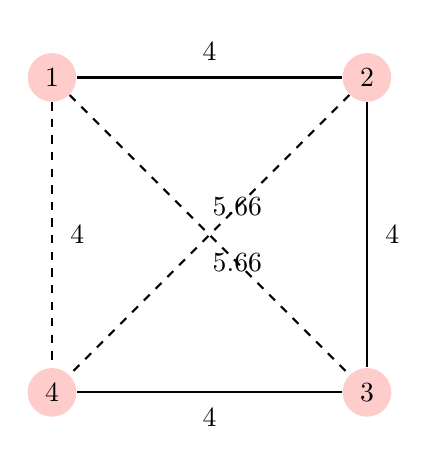
\begin{tikzpicture}
  [scale=1,auto=left,every node/.style={circle,fill=red!20}]
  \tikzstyle{weight} = [fill=none]
  \node (n1) at (1,9)  {1};
  \node (n2) at (5,9)  {2};
  \node (n3) at (5,5)  {3};
  \node (n4) at (1,5)  {4};
  \foreach \source /\dest /\weight in {n1/n2/4,n2/n3/4,n3/n4/4} 
   \draw[thick] (\source) --node[weight] {$\weight$}  (\dest);
\foreach \source /\dest /\weight in {1/3/1} place \weight above of=\path;
  \foreach \source /\dest /\weight in {n1/n4/4,n1/n3/5.66,n2/n4/5.66} 
   \draw[color=black,thick,dashed] (\source) --node[weight] {$\weight$}  (\dest);
\foreach \source /\dest /\weight in {1/3/1} place \weight below of=\path;
  \end{tikzpicture}
\caption{A minimum spanning tree representation with a total weight of~12 for a set of four points in the plane; here, edges not part of the minimum spanning tree are shown as dashed lines}\label{11g9}
\end{center}
\end{figure}

\begin{figure}
\begin{center}
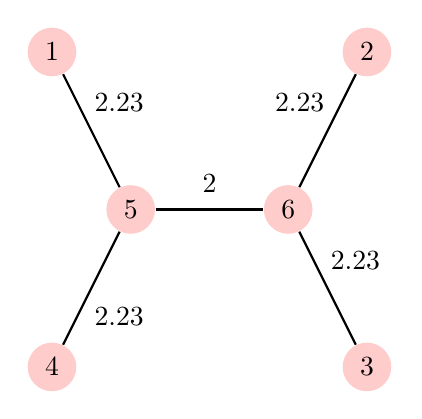
\begin{tikzpicture}
  [scale=1,auto=left,every node/.style={circle,fill=red!20}]
  \tikzstyle{weight} = [fill=none]
  \node (n1) at (1,9)  {1};
  \node (n2) at (5,9) {2};
  \node (n3) at (5,5)  {3};
  \node (n4) at (1,5)  {4};
  \node (n5) at (2,7) {5};
  \node (n6) at (4,7) {6};
  \foreach \source /\dest /\weight in {n1/n5/2.23,n5/n6/2,n6/n2/2.23,n6/n3/2.23,n5/n4/2.23} 
   \draw[thick] (\source) --node[weight] {$\weight$}  (\dest);
\foreach \source /\dest /\weight in {1/3/1} place \weight below of=\path;
 
  \end{tikzpicture}
\caption{A minimum Steiner tree for the set of four points or vertices shown in Figure~\ref{11g9}; here, Steiner points are vertices~5 and~6}\label{11g10}
\end{center}
\end{figure}

Another ghost named Urpur had been eavesdropping on Rishnak and Ajur. Urpur wanted to show that he was smarter than both Rishnak and Ajur, so he interrupted and said, ``I have an even smarter approach. There is a spanning tree called the Steiner tree\footnote{Named after the Swiss mathematician Jakob Steiner} wherein one is allowed to add Steiner points or vertices that were not present in the original problem. With a clever addition of Steiner points, I can find a spanning tree that is better than the one Ajur found.''

Urpur clapped his hands and a new graph appeared [Figure~\ref{11g10}]. Urpur said, ``You see?''

Rishnak was impressed with Urpur's solution, but sensing that Ajur was feeling jealous of Urpur, Rishnak said, ``Not bad, Urpur. I am sure Ajur would have also come to this solution if I had asked him.''

Ajur nodded in agreement.

%%\newpage
\subsection*{Question for the ninth day}
Rishnak said, ``It is time now for Ajur to try and answer the question for the ninth day. It has multiple parts.''

Ajur's eyes opened wide in excitement.

Rishnak continued, ``Consider a complete graph with with eight vertices and 28~edges. Of these edges, 14 of them have a weight of~1, while the other 14~edges all have a weight of~10. First, how must you assign the weights so as to achieve the smallest possible minimum weight spanning tree? Second, how must you assign the weights so as to achieve the opposite, the largest possible minimum weight spanning tree?''

\textit{Before you turn the page, try to come up with an answer of your own!}

\newpage
\subsection*{Answer for the ninth day}
Ajur started with the first part. He said, ``If there is a cycle that visits all of the vertices---so a cycle of length~8---and each edge weight in the cycle is~1, then the minimum spanning tree has a weight of~7. We can't go smaller than that.''

Rishnak smiled and said, ``Correct. And for the second part?''

Before Ajur could answer, Urpur said, ``The second part is the real question. And the answer is---''

Ajur jumped up and said, ``The answer is~25. The largest minimum spanning tree will have a total weight of~25.''

Rishnak said, ``And how do you know that?''

Ajur said, ``All of the edges incident at a vertex must be of weight~10 or else we would select an edge of length~1 instead.  Since there are eight vertices, the degree of each vertex must be~7, so two of the graph's vertices can entirely have incident edges of weight~10. That uses up the~14 edge weights of~10, and gives us a minimum spanning tree with a total weight of~$10+10+1+1+1+1+1$, which is~$25$.''

Rishnak smiled.

Urpur said, ``That's what I was going to say!''

Rishnak laughed and decided to call it a night.

Jura barked. He was happy now to get Ajur's attention and jumping with joy, left with Ajur.
